\section{Phương pháp đề xuất}\label{sec:method}
\frame{\tableofcontents[currentsection]}

\subsection{Ý tưởng thực hiện luận văn}
\begin{frame}{Ý tưởng thực hiện luận văn}
    \begin{itemize}
        \item Luận văn kế thừa kết quả nghiên cứu của Lele Chen và cộng sự \cite{chen2019}
        \begin{itemize}
            \item Nắm rõ ý tưởng của tác giả và quy trình công nghệ
            \item Thực nghiệm lại mô hình tạo sinh hình ảnh của tác giả
        \end{itemize}
        \item Luận văn cũng kết hợp có chỉnh sửa cách chuẩn hóa cột mốc gương mặt từ nghiên cứu Generating Talking Face Landmarks from Speech\cite{gen_face_landmark} để cho kết quả tạo sinh tốt hơn
        \begin{itemize}
            \item Cột mốc gương mặt phải có cùng kích thước
            \item Vị trí của mắt, mũi, miệng trên cột mốc gương mặt cần phải được chuyển về một vị trí đồng nhất cho mọi khung hình
            \item Hạn chế việc ảnh hưởng của đặc điểm nhận dạng của khuôn mặt lên cột mốc gương mặt
        \end{itemize}
    \end{itemize}
\end{frame}

\begin{frame}{Ý tưởng thực hiện luận văn}
    \begin{figure}[H]
        \centering
        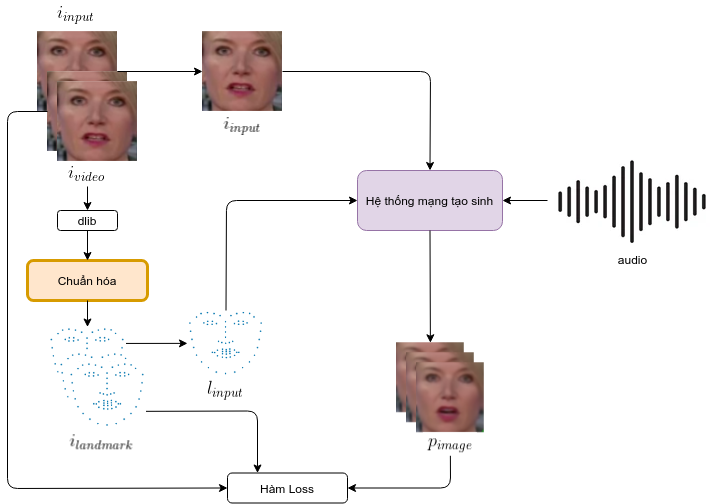
\includegraphics[width=9.5cm]{images/processing-contrib.png}
        \label{fig:processing-contrib}
        \caption{Chuẩn hóa cột mốc gương mặt trước khi đưa vào mạng}
    \end{figure}
\end{frame}

\subsection{Tiền xử lý dữ liệu}
\begin{frame}{Tiền xử lý dữ liệu}
    Ta mong muốn đầu vào của mạng là một cột mốc gương mặt chung nhất và không bị ảnh hưởng bởi đặc điểm mặt người trên video. Vì vậy, ta cần tạo ra cột mốc gương mặt chuẩn bằng cách lấy trung bình cộng của nhiều cột mốc trong nhiều video khác nhau
    \begin{figure}[H]
        \centering
        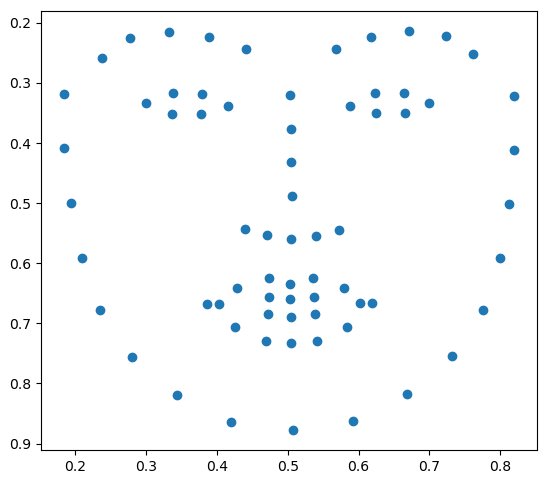
\includegraphics[width=6cm]{images/standard_landmark.png}
        \label{fig:standard_landmark}
        \caption{Cột mốc gương mặt chuẩn}
    \end{figure}
\end{frame}

\begin{frame}{Tiền xử lý dữ liệu}
    Ý tưởng chuẩn hóa cột mốc gương mặt
    \begin{itemize}
        \item Chuyển vùng mắt của cột mốc gương mặt trong video về vị trí tương ứng trên cột mốc chuẩn
        \item Tìm đạo hàm của chuỗi cột mốc gương mặt, tính tổng cộng dồn của đạo hàm này để tìm ra sự thay đổi của cột mốc tại thời điểm $t$ so với thời điểm ban đầu
        \item Chuyển sự thay đổi này lên cột mốc gương mặt chuẩn
        \item Điều chỉnh lại vùng mũi, miệng của cột mốc gương mặt vừa được tính toán ra bằng các phép biến đổi Affine để khớp hơn với cột mốc chuẩn
    \end{itemize}
\end{frame}

\begin{frame}{Tiền xử lý dữ liệu}
    Với cách chuẩn hóa nêu trên, ta có thể đưa chuyển động của cột mốc gương mặt ban đầu lên cột mốc gương mặt chuẩn, với các góc độ quay khác nhau của video và loại bỏ đặc điểm gương mặt người nói
    \begin{figure}[H]
        \centering
        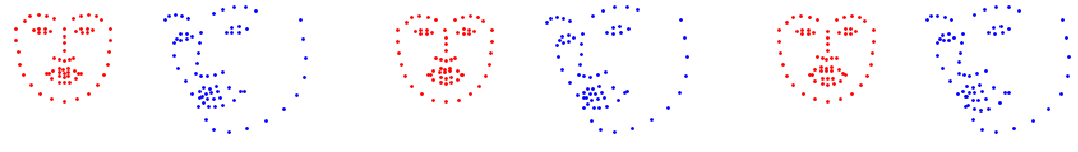
\includegraphics[width=11cm]{images/standardized_landmark.png}
        \label{fig:standardized_landmark}
        \caption{Kết quả chuẩn hóa cột mốc gương mặt. Cột mốc ban đầu (xanh), chuẩn hóa (đỏ)}
    \end{figure}
\end{frame}

\begin{frame}{Tiền xử lý dữ liệu}
    Nhờ việc điểu chỉnh lại cột mốc gương mặt ở vùng mũi và miệng, vùng miệng của gương mặt được đưa về gần nhất với vùng miệng của cột mốc chuẩn, vì vậy tất cả các cột mốc được tính toán sẽ có cùng một kích thước vùng miệng, giúp cho mạng dễ học hơn
    \begin{figure}[H]
        \centering
        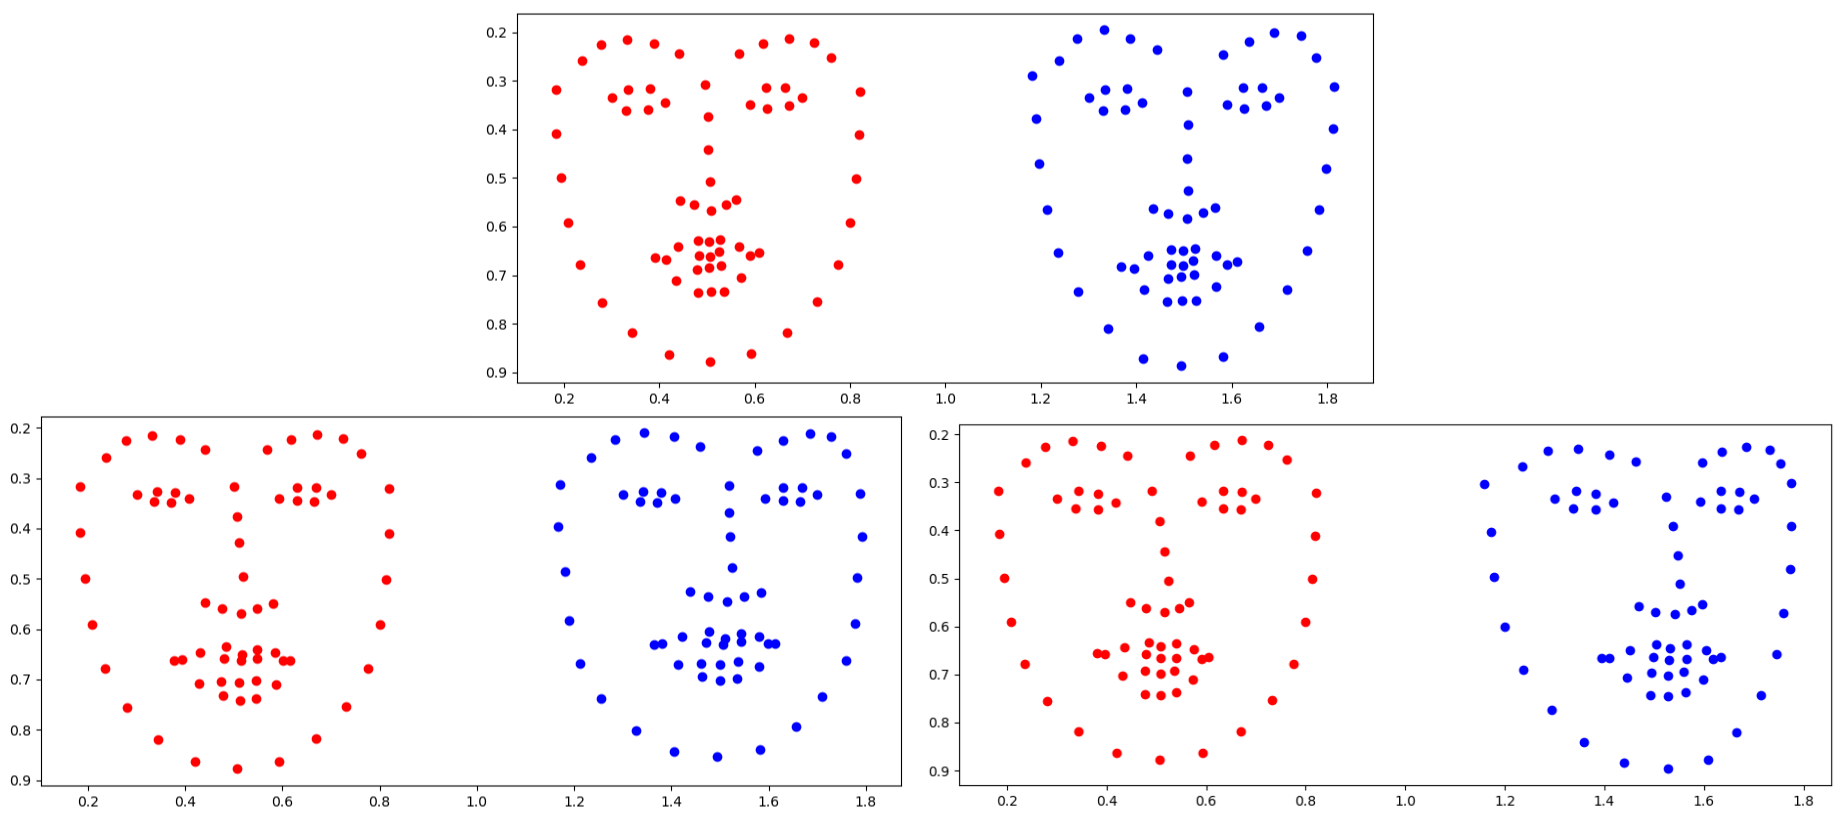
\includegraphics[width=11cm]{images/landmark_alignment.png}
        \label{fig:landmark_alignment}
        \caption{Kết quả chuẩn hóa vùng miệng. Cột mốc chưa chuẩn hóa (xanh), chuẩn hóa (đỏ)}
    \end{figure}
\end{frame}

\begin{frame}{Tiền xử lý dữ liệu}
    Dựa vào cột mốc gương mặt được trích xuất và chuẩn hóa, ta cũng sử dụng phép biến đổi Affine trên các khung hình trong video, để đưa gương mặt trên hình về vị trí khớp nhất với cột mốc chuẩn
    \begin{figure}[H]
        \centering
        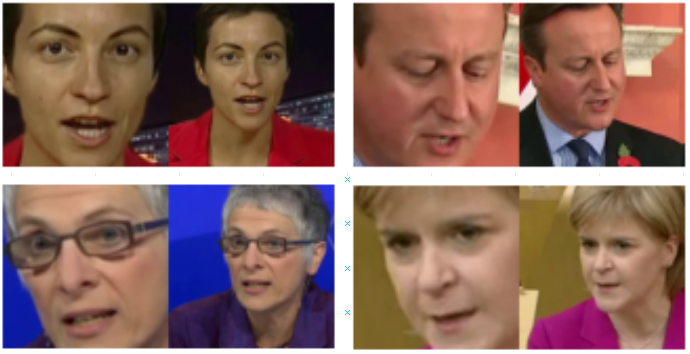
\includegraphics[width=9cm]{images/preprocessed-image.png}
        \label{fig:preprocessed-image}
        \caption{Kết quả chuẩn hóa hình ảnh}
    \end{figure}
\end{frame}

\subsection{Các tập dữ liệu được sử dụng}
\begin{frame}{Các tập dữ liệu được sử dụng}
Tập dữ liệu GRID: Tập dữ liệu chứa 1000 câu, được nói bởi 34 người khác nhau. Như vậy, tập dữ liệu này chứa 34000 video với chất lượng cao, mỗi video có độ dài 3 giây.

    \begin{figure}[H]
        \centering
        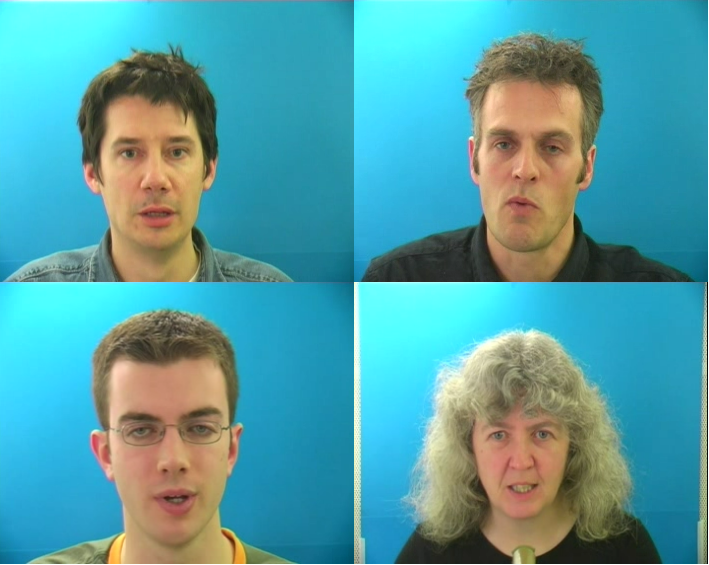
\includegraphics[width=7cm]{./images/grid.png}
        \caption{Ảnh trích xuất từ các video trong tập dữ liệu GRID}
    \end{figure}
\end{frame}

\begin{frame}{Các tập dữ liệu được sử dụng}
Tập dữ liệu LRW: Tập dữ liệu chứa hơn 1 triệu video khác nhau, mỗi video có độ dài 1.16 giây, gồm 29 khung hình. Những video này được chia làm 1000 từ vựng, mỗi từ vựng được nói bởi hơn 1000 người khác nhau. Tổng cộng, tập dữ liệu LRW chứa gần 1000 giờ video.
    \begin{figure}[H]
        \centering
        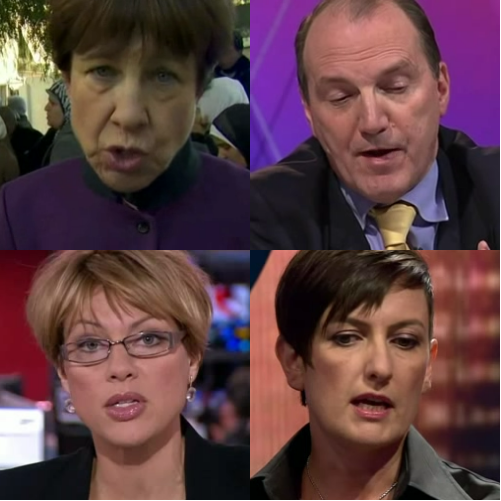
\includegraphics[width=5cm]{./images/lrw.png}
        \caption{Ảnh trích xuất từ các video trong tập dữ liệu LRW}
    \end{figure}
\end{frame}

\subsection{Các độ đo được sử dụng}
\begin{frame}{Các độ đo được sử dụng}
Độ đo SSIM: Là độ đo sự tương đồng về mặt cảm quan giữa hai hình ảnh, dựa trên ba yếu tố là độ tương phản, ánh sáng, và cấu trúc của ảnh. Càng gần về 1, ảnh tạo sinh càng giống với ảnh gốc.
\begin{equation}
SSIM(x,y) = \frac{(2\mu_x\mu_y + C_1) + (2 \sigma _{xy} + C_2)} 
    {(\mu_x^2 + \mu_y^2+C_1) (\sigma_x^2 + \sigma_y^2+C_2)}
\label{eq:SSMI}
\end{equation}
Với:
\begin{itemize}
    \item $\mu_x$, $\mu_y$: trung bình của các điểm ảnh trong cửa sổ
    \item $\sigma_x^2$, $\sigma_y^2$: variance của các điểm ảnh trong cửa sổ
    \item $C_1$, $C_2$: hằng số để ổn định phép chia
\end{itemize}
\end{frame}

\begin{frame}{Các độ đo được sử dụng}
Độ đo CPBD: Là độ đo thể hiện sự sắc nét của hình ảnh, là xác suất tích lũy của các cạnh trên ảnh nếu không được xem là cạnh mờ (blur). Một cạnh được xem là mờ khi nó có độ dày quá lớn, vượt qua độ dày được quy định là mờ $W_{JNB}$
\begin{equation}
CPBD = P(P_{BLUR} < P_{JNB}) = \sum^{P_{BLUR} = P_{JNB}}_{P_{BLUR} = 0}(P_{BLUR})
\label{eq:CPBD}
\end{equation}
Với:
\begin{itemize}
    \item $P_{BLUR}$: xác suất một cạnh bị mờ. $P_{BLUR} = 1 - e^{-(\frac{W_{e(i)}}{W_{JNB}(e_i)})^\beta}$
    \item $W_{JNB}$: Độ dày cạnh quy định là mờ
    \begin{itemize}
        \item $W_{JNB} = 5$ nếu độ tương phản nhỏ hơn hoặc bằng 50
        \item  $W_{JNB} = 3$ nếu độ tương phản lớn hơn 50
    \end{itemize}
\end{itemize}
\end{frame}

\subsection{Môi trường thí nghiệm}
\begin{frame}{Môi trường thí nghiệm}
\begin{table}[h]
    \centering
    \begin{tabular}{c | c | c}
    \hline 
    &\textbf{Máy A} & \textbf{Máy B}\\
    \hline
    \textbf{CPU} & Intel Xeon & Intel Core I5 8600K\\
    \textbf{Bộ nhớ} & 24GB & 32GB\\
    \textbf{GPU} & NVIDIA TESLA V100 & NVIDIA Geforce RTX 3070\\
    \textbf{Ổ cứng} & 160GB SSD & 768GB NVME SSD + 2TB HDD\\
    \textbf{OS} & N/A(Colab Pro) & Ubuntu 20.04\\
    \textbf{Ngôn ngữ} & Python 3.7 & Python 3.7\\
    \textbf{Framework} & Pytorch 1.8 & Pytorch 1.8\\
    \hline
    \end{tabular}
    \caption{Các môi trường được sử dụng trong việc tiền xử lý dữ liệu, huấn luyện và thực hiện thí nghiệm}
    \label{table:hardware}
\end{table}
\end{frame}

\subsection{Thực hiện thí nghiệm}
\begin{frame}{Thực hiện thí nghiệm}
Quá trình huấn luyện mạng tạo sinh cột mốc gương mặt:
\begin{table}[h]
    \centering
    \begin{tabular}{c | c | c}
    \hline 
    &\textbf{GRID} & \textbf{LRW}\\
    \hline
    \textbf{Bộ tối ưu} & Adam & Adam\\
    \textbf{Kích thước bó} & 100 & 100\\
    \textbf{Hệ số học} & 0.001 & 0.0002\\
    \textbf{Thời gian huấn luyện} & 5 phút & 70 phút\\
    \textbf{$\mathcal{L}_{landmark}$} & $4.9200 \times 10^{-4}$ & $2.012 \times 10^{-4}$\\
    \hline
    \end{tabular}
    \caption{Chi tiết huấn luyện mạng tạo sinh cột mốc gương mặt. Giá trị mất mát (trên tập kiểm thử) và thời gian huấn luyện được ghi nhận tại vòng lặp cho ra mô hình tối ưu}
    \label{table:landmark_decoder_training_detail}
\end{table}
\end{frame}

\begin{frame}{Thực hiện thí nghiệm}
Quá trình huấn luyện mạng GANs:
    \begin{table}[h]
    \centering
    \begin{tabular}{c | c | c}
    \hline 
    &\textbf{GRID} & \textbf{LRW}\\
    \hline
    \textbf{Bộ tối ưu} & Adam & Adam\\
    \textbf{Kích thước bó} & 12 & 17\\
    \textbf{Hệ số học} & 0.0002 & 0.0002\\
    \textbf{Thời gian huấn luyện} & 5 giờ 20 phút & 250 giờ\\
    \textbf{$\mathcal{L}_{pix}$} & $4.1575 \times 10^{-2}$ & $6.8502 \times 10^{-2}$\\
    \textbf{$\mathcal{L}_{gans-dis}$} & $0.9964$ & $0.6931$\\
    \textbf{$\mathcal{L}_{gans-landmark}$} & $7.6990 \times 10^{-2}$ & $5.2412 \times 10^{-2}$\\
    \textbf{$\mathcal{L}$} & $1.4892$ & $1.4306$\\
    \hline
    \end{tabular}
    \caption{Chi tiết huấn luyện mạng GANs. Giá trị mất mát (trên tập kiểm thử) và thời gian huấn luyện được ghi nhận tại vòng lặp cho ra mô hình tối ưu}
    \label{table:gans_training_detail}
\end{table}
\end{frame}

